\section{Decision Trees}
\label{sec:dt}


\subsection{J48 Algorithm}
\label{sec:dt:j48}
\subsubsection{Variation in performance with size of the training and testing sets}
\raggedright\underline{Cross\-Validation Accuracy On Different Files}


We executed the J48 Algorithm on fer2017-training/testing and fer2017-training/testing-happy using 10 fold cross validation. The full data set was used with the only variation being moving  9000 or 16000 from the training set to the testing set. This was done to see the effect of different sizes of training and testing set on the accuracy. The table below displays the data collected.

J48 is used to generate a decision tree. It is a supervised learning algorithm which requires a data set to be used as the training example. The algorithm analyses the training set and builds a classifier that can be used to correctly classify testing instances\autocite{octaviansima2013}. Some advantages are it is easy to implement and is easy to interpret. Some disadvantages are that the algorithm easily generalises and over fits to the training set. This is demonstrated by a small variation of data can lead to a different tree being constructed meaning that instead of training for the situation, it trains for the data in the training set.


\begin{figure}[hbt!]
	\centering
      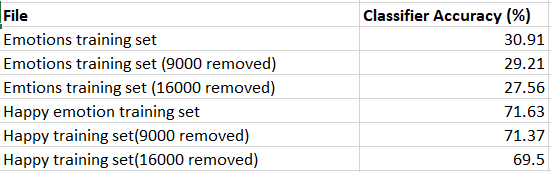
\includegraphics[width=0.7\textwidth]{imgs/J48/CVTraining.png} \\
	\caption{Cross validation accuracy on the training files}
	\label{fig:dt:CVTraining_table}
\end{figure}

Cross validation can be used to find out if the data set is overfitted to the training data, this will be discussed further in \ref{sec:dt:tts}. In figure \ref{fig:dt:CVTraining_table} the data displays that the accuracy of the J48 algorithm on training files with all emotion decreases from \textbf{'30.91\%'} to\textbf{ '27.56\%'} when the data set is reduced incrementally. The computation time also decreased when the data set was reduced. The standard deviation of the training set on all emotions was relatively low apart from happy. 

Happy had both the highest TP and highest FP rate, this is due to Happy being the largest emotion in the data set. When observing the happy data, the effect of reducing the data set did not greatly impact the classifiers accuracy. The greatest difference is the set with 9000 thousand removed and the set of 16000 thousand removed decreasing from \textbf{'71.37\%'} to \textbf{'69.5\%'}.

\begin{figure}[hbt!]
	\centering
      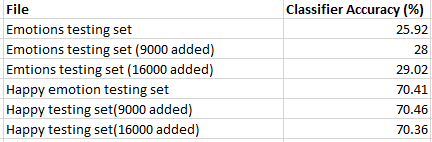
\includegraphics[width=0.7\textwidth]{imgs/J48/CVTesting.PNG} \\
	\caption{Cross validation accuracy on the testing files}
	\label{fig:dt:CVTesting_table}
\end{figure}


Cross validation being executed on the testing data sets displays the opposite when discussing the full emotion list compared to the training data. The accuracy increases from \textbf{'25.92\%'} to\textbf{ '29.02\%'}. But the same remains when looking at the happy testing set with all tests concluding at around\textbf{'70\%'}.

\raggedright\underline\raggedright\underline{Testing on different test sets}

One of the main disadvantages of J48 is highlighted when testing on different test sets.

\begin{figure}[hbt!]
	\centering
      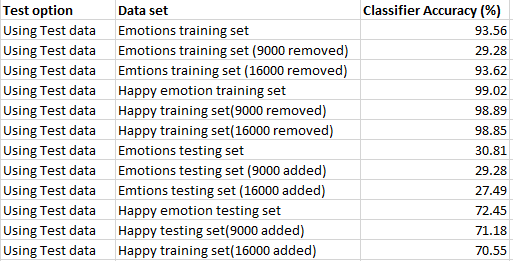
\includegraphics[width=0.7\textwidth]{imgs/J48/TestingOnDifferentTestSets.PNG} \\
	\caption{Accuracy using J48 on different test data}
	\label{fig:dt:Testingondifftests}
\end{figure}
when testing on unseen data, the test datasets, J48 has low classifier accuracy relatively similar to the accuracies found in cross validation

\label{sec:dt:tts}
\raggedright\underline{Testing Different Parameters}


\raggedright\underline{Variation in performance with size of the training and testing sets}

BLANK TEXT HERE
\newline

\raggedright\underline{Variation in performance with varying learning parameters in Random Forest}

BLANK TEXT HERE
\newline

\raggedright\underline{Variation in performance according to different metrics}



\subsection{Random Forest}
\label{sec:dt:rf}
For this coursework we had to select one other decision tree algorithm. The algorithm we decided to use was the Random Forest algorithm \autocite{Breiman2001}. This was selected due to the coursework's focus on overfitting. The Random Forest algorithm helps to fix the overfitting that J48 is prone to. The complexity of a classifier such as J48 can reach a point where it is negatively impacted by overfitting. The nature of Random Forest algorithm means that increased iterations do not lead to a point where it is perfectly optimised for the training set and therefore harming the accuracy of the testing set. Machine Learning algorithms should be well optimised for unseen test data, rather than training data. The algorithm in WEKA is based on Breiman's implementation \autocite{Breiman2001}. It combines bagging with a random selection of features. Bagging combines the classifications of randomly generated subsets of the main training set. Random selection of features further reduces overfitting by allowing the algorithm to only select a set number of randomly chosen features. Each iteration in WEKA produces a new decision tree. An instance(row) in the data set is classified by finding the mode class of all the trees. For example, if you have 10 iterations there will be 10 decision trees. If 6 trees classify the pixel attributes as Happy then it will be classified as happy because it is the highest mode. We discovered that random forest consistently performed better than J48 with quicker compile time.

Using Python we automated numerous different experiments, totalling 688 executions of the algorithm on different testing options and parameters. These results are summarised in 6 tables found in the Appendix (section 5.3.1). We ran the algorithm on 16 different test options. The required ones were crossfold on the training set and using the test sets with varying number of instances (totalling 8 different test options). I additionally ran crossfold on the test set (smaller data comparison) and used the training sets as a test set (to use in discussion of overfitting). Below is a summary of the analysis found.  

\raggedright\underline{Variation in performance with size of the training and testing sets}

\begin{enumerate}
  \item Larger data sets perform better. The classifier accuracy using crossfold on the original training set (28709 instances) was consistently higher than the original test set (7178 instances). This was true for both Happy and All emotions. 10 crossfold validation on Happy Training set produced 78.24\% accuracy whereas on the Test set it produced 76.95\%. The Emotions data saw a much larger decrease in accuracy when using the test set dropping from 44.25\%(training set) to 37.57\%(test set). An increase in data improves the training of the random forest algorithm.
  \item Using the test set rather than crossfold validation produces higher accuracy. This is expected as crossfold validation gives a more realistic measure of how well a model will classifier unseen data.
  \item Moving instances from the training set to the test set reduces accuracy in both Happy and all emotions data set. This is expected as the classifier has less data to build a model which will be tested on more data. More instances in the test data means more cases for the model to handle. Logically, the more cases a model has to handle the lower the chance of classification. Furthermore, the change in ratio of training to test data means that after adding 16000 instances to the test set you are in fact using a test set that is larger than the data used to train. The significance of this is that smaller training set will be prone to more bias. This model with increased bias towards the training data is now tested on a larger quantity of data with did not impact the bias. The decrease in accuracy is supported by the results. Using the original test set the classifier built on emotions training data produced 45.56\%. Moving 9000
  
  
  \item Using the training sets for testing consistently produces accuracy close to 99\%. This is not necessarily a good thing as it means the model is very optimised for the training data when it should be optimised for unseen data.  
\end{enumerate}


\raggedright\underline{Variation in performance with varying learning parameters in Random Forest}

BLANK TEXT HERE
\newline

\raggedright\underline{Variation in performance according to different metrics }

BLANK TEXT HERE
\newline










\subsection{User Classifiers}
\label{sec:dt:uc}
After running the \textbf{Random Forest} experiments we constructed a semi-manual tree with the \textbf{500, 1000, 1250, 1500 and 2000} pixel attributes selected on the \textbf{emotions test set.} This then had the \textbf{Random Forest} classifier applied to the leaf node as seen in \textbf{figure \ref{fig:dt:semi_manual_random_forrest}}. We applied this to the non-split training and testing data, using the `\textbf{Supplied test set}' option, as well as the `\textbf{Cross-validation}' with 10 folds specified. The settings used for the classifier in the semi-manual tree is shown in \textbf{figure \ref{fig:appendix:classifier:rfucs}} at \textbf{appendix \ref{sec:appendix:classifier:rfucs}} and were the default for \textbf{Random Forest}.

\begin{figure}[hbt!]
	\centering
      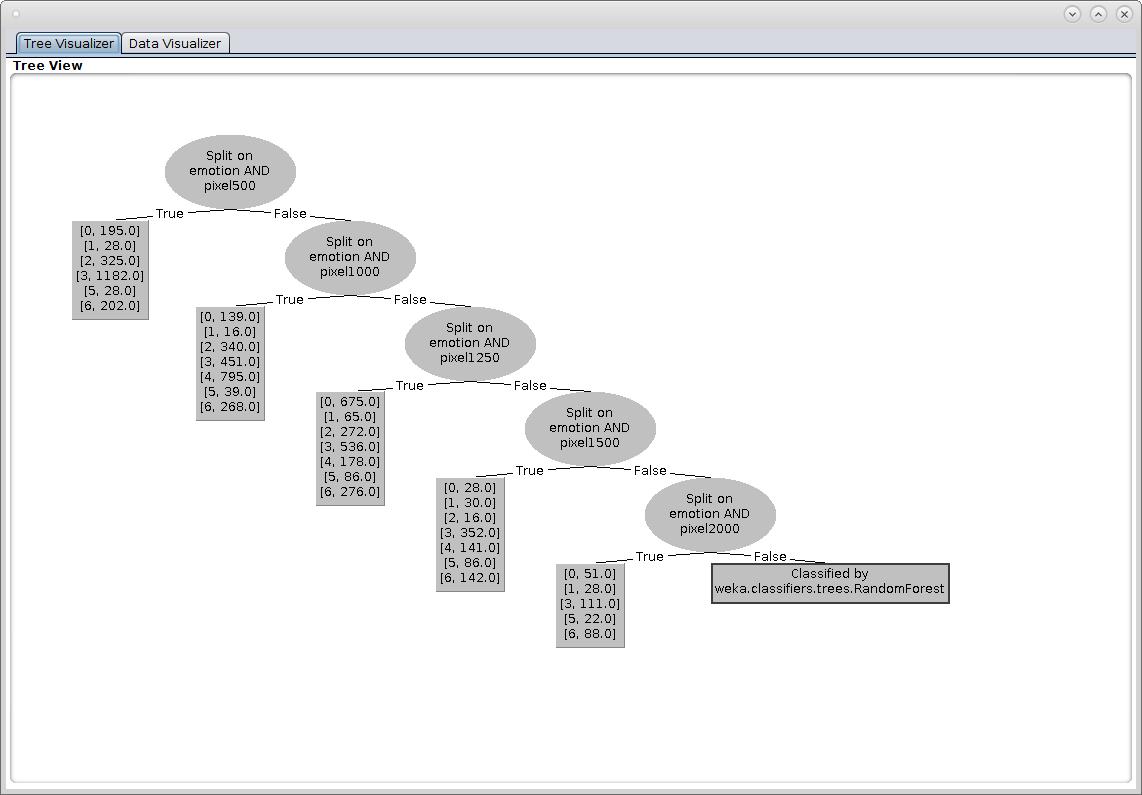
\includegraphics[width=0.6\textwidth]{imgs/userClassifier/noSplit/all/Train-and-Test/tree_settings_with_classifier.png} \\
	\caption{Semi-Manual Tree with Random Forrest Classifier}
	\label{fig:dt:semi_manual_random_forrest}
\end{figure}


When selecting points to be removed from our chosen pixels we aimed to select edge cases, where data points appear as \textit{anomalies}. This focused the data into larger clumps, narrowing an emotion's correlation with the pixel values. Looking at \textbf{figure \ref{fig:dt:supplied_test_set:pixel500},}  red emotion \textbf{1} highlights value points which were sparsely grouped at the top and bottom of the pixel value range. This was done consistently with each emotion on the specified pixels \textbf{500, 1000, 1250, 1500 and 2000}. 

\FloatBarrier
\begin{figure}[hbt!]
	\centering
      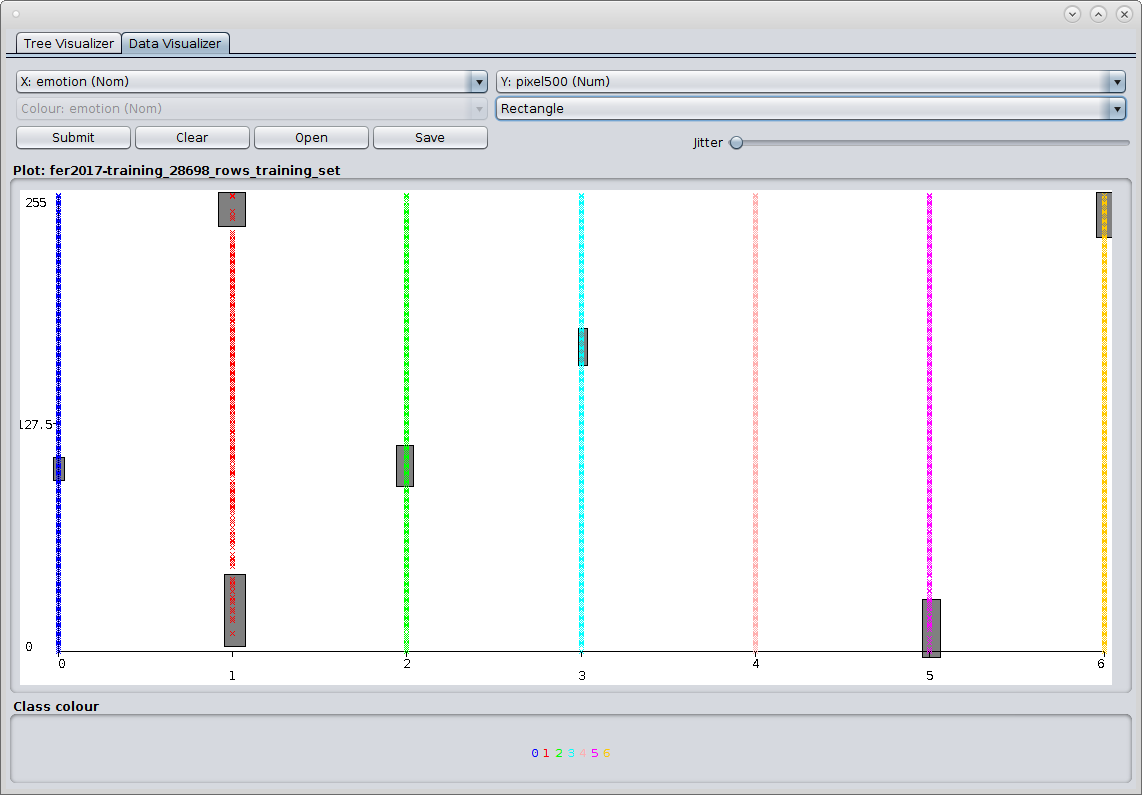
\includegraphics[width=0.6\textwidth]{imgs/userClassifier/noSplit/all/Train-and-Test/500.png} \\
	\caption{Pixel 500 Selected Pixel Values}
	\label{fig:dt:supplied_test_set:pixel500}
\end{figure}

\subsubsection{Supplied Test Set}
\label{sec:dt:uc:sts}

Building the classifier with \textbf{fer2017-training\_28698\_rows\_training\_set.arff} and supplying test data with \textbf{fer2017-testing\_rows\_testing\_set.arff} produced an accuracy of \textbf{42.59\%} (\textbf{Figure \ref{fig:dt:uc:results}}) compared to \textbf{45.56\%} from the default \textbf{Random Forest} experiment (\textbf{Appendix \ref{sec:appendix:charts_tables}, figure \ref{fig:randomforest_main}}). The \textit{FP} rates are consistently lower for the semi-manual User Classifier (UC Random Forest) compared to the default classifier of the \textbf{Random Forest} algorithm. The only exception of this can be seen for the \textbf{Happy (3)} emotion which has a higher \textit{FP} rate at\textit{ 0.364} compared to \textit{0.233} (\textbf{Table \ref{table:uc:randForest_vs_UCrandForest_tpfp}}).

\FloatBarrier
\begin{figure}[hbt!]
	\centering
      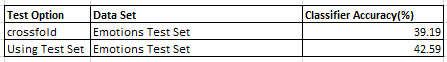
\includegraphics[width=0.75\textwidth]{imgs/userClassifier/noSplit/all/userclassifier_accuracy_results.PNG} \\
	\caption{Cross-validation and Using test set results with User Classifiers and Random Forest}
	\label{fig:dt:uc:results}
\end{figure}





\FloatBarrier
\begin{table}[htb!]
\begin{center}
 \begin{tabular}{||P{0.105\linewidth}|P{0.1\linewidth}|P{0.1\linewidth}|P{0.1\linewidth}|P{0.1\linewidth}|P{0.1\linewidth}|P{0.1\linewidth}|P{0.1\linewidth}||} 
 \hline
 \textbf{TP}-\textit{FP} Rates 
 & \textbf{Angry (0)} 
 & \textbf{Disgust (1)} 
 & \textbf{Fear (2)} 
 & \textbf{Happy (3)} 
 & \textbf{Sad (4)} 
 & \textbf{Surprise (5)} 
 & \textbf{Neutral (6)} 
 
 \\ \hline\hline
 
 \textbf{Random Forest} 
 & \textbf{0.193}-\textit{0.037} 
 & \textbf{0.318}-\textit{0.0} 
 & \textbf{0.259}-\textit{0.046} 
 & \textbf{0.804}-\textit{0.364} 
 & \textbf{0.335}-\textit{0.106} 
 & \textbf{0.602}-\textit{0.033} 
 & \textbf{0.356}-\textit{0.099}
 
 \\  \hline
 
 \textbf{UC Random Forest} 
 & \textbf{0.18}-\textit{0.039} 
 & \textbf{0.255}-\textit{0.0} 
 & \textbf{0.289}-\textit{0.087} 
 & \textbf{0.625}-\textit{0.233} 
 & \textbf{0.352}-\textit{0.129} 
 & \textbf{0.645}-\textit{0.066} 
 & \textbf{0.387}-\textit{0.151}
 
 \\ \hline
 
 \hline
\end{tabular}
\caption{Random Forest vs. User Classifier Random Forest \textbf{TP}-\textit{FP} Rates}
\label{table:uc:randForest_vs_UCrandForest_tpfp}
\end{center}
\end{table}






\FloatBarrier
\subsection{Comparing J48 and Random Forest}